\section{Grad-CAM}
Grad-CAM\cite{selvaraju2017grad} (Gradient-weighted Class Activation Mapping) is a white box method, it requires insight into the convolutional neural network architecture and is therefore only applicable on CNNs. The method generates a heat map similar to RISE. Figure \ref{grad_cam_dog} and Figure \ref{grad_cam_cat} show an example output of Grad-CAM.

\begin{figure}[H]
    \centering
    \begin{subfigure}{.5\textwidth}
        \centering
        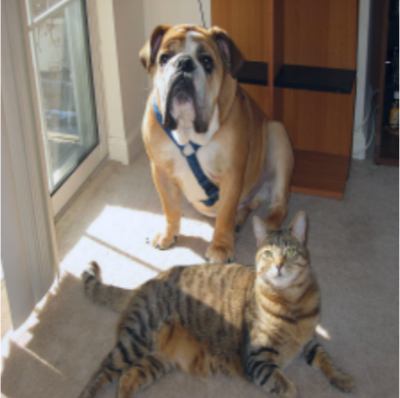
\includegraphics[width=0.7\linewidth]{chapters/02_methods/images/grad-cam-original.png}
        \caption{Original image}
    \end{subfigure}\hfill%
    \begin{subfigure}{.5\textwidth}
        \centering
        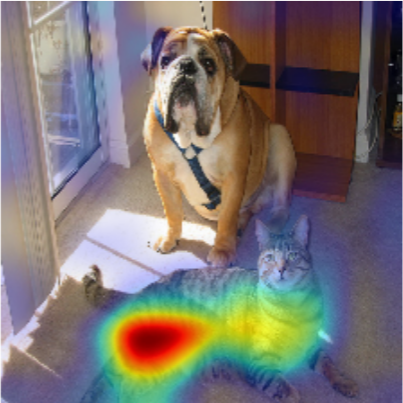
\includegraphics[width=0.7\linewidth]{chapters/02_methods/images/grad-cam-cat.png}
        \caption{Grad-CAM explanation for class cat}
    \end{subfigure}
    \caption{Grad-CAM applied on an image with multiple valid classes. Explanation for class cat.}
    \label{grad_cam_cat}
\end{figure}

\begin{figure}[H]
    \centering
    \begin{subfigure}{.5\textwidth}
        \centering
        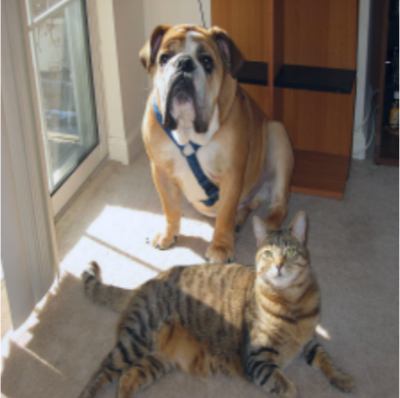
\includegraphics[width=0.7\linewidth]{chapters/02_methods/images/grad-cam-original.png}
        \caption{Original image}
    \end{subfigure}\hfill%
    \begin{subfigure}{.5\textwidth}
        \centering
        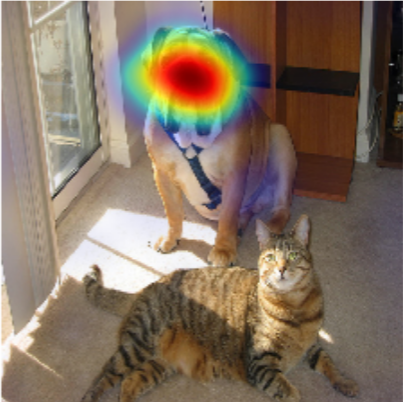
\includegraphics[width=0.7\linewidth]{chapters/02_methods/images/grad-cam-dog.png}
        \caption{Grad-CAM explanation for class dog}
    \end{subfigure}
    \caption{Grad-CAM applied on an image with multiple valid classes. Explanation for class dog.}
    \label{grad_cam_dog}
\end{figure}

The main parameter for this method is which convolutional layer of the neural network that should be analyzed. Figure \ref{grad_cam_explanation} shows a schematic of the inner working of Grad-CAM for a layer: The feature map of the specified convolutional layer is extracted. Every channel of the feature map is weighted, based on how much it influences the final output value of the network for a specific class. Finally, the weighted channels are summed up and converted into a heat map.

\begin{figure}[H]
\centering
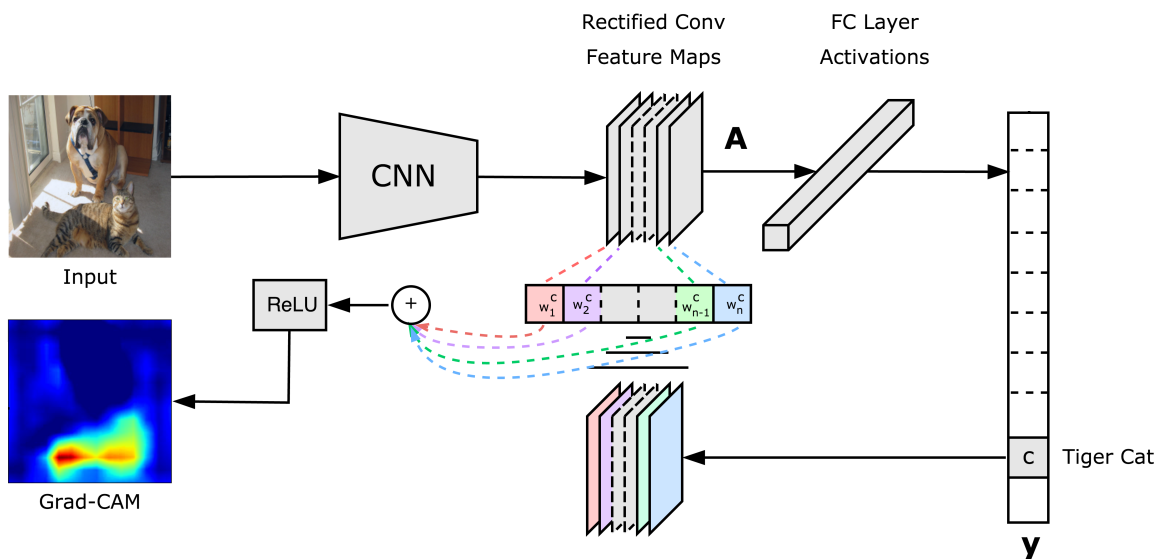
\includegraphics[width=12cm]{chapters/02_methods/images/grad-cam.png}
\caption{Grad-CAM in action: The feature map of a specific network layer is extracted, each channel weighted by the activation of the expected class, then summed up and converted into a heat map}
\label{grad_cam_explanation}
\end{figure}

